\documentclass[a4paper,12pt]{article}

\usepackage{amsmath,amssymb,amsfonts,gensymb,mathtext,enumerate,float,cite}
\usepackage[T2A]{fontenc}
\usepackage[utf8]{inputenc}
\usepackage[english,russian]{babel}
\usepackage{indentfirst}
\usepackage[unicode=true]{hyperref}
\usepackage{multirow}
\usepackage{array}	
\usepackage[dvips]{graphicx}
\usepackage{xymtexpdf}
\usepackage{caption}
\usepackage{cmap}
\graphicspath{{images/}}



\usepackage{setspace}
% полуторный интервал
\onehalfspacing
\usepackage[12pt]{extsizes}

\hypersetup{
pdfborder={0 0 0},
pdfauthor={Khaibrakhmanov Artur Ilnurovich},
pdftitle={Thesis},
}

\usepackage{geometry}\geometry{left=2cm}
\geometry{right=2cm}
\geometry{top=2cm}
\geometry{bottom=2.5cm}

%\numberwithin{equation}{section}
%\numberwithin{figure}{section}
%\numberwithin{table}{section}

\setcounter{tocdepth}{4}
\setcounter{secnumdepth}{4}

\RequirePackage{caption}
\usepackage[labelsep=period]{caption}
%\DeclareCaptionLabelSeparator{defffis}{ -- }
\captionsetup{justification=centering}%,labelsep=defffis}
\usepackage{subfigure}
%\usepackage{subcaption}
\renewcommand{\thesubfigure}{(\asbuk{subfigure})}
\begin{document}
\righthyphenmin=20
\renewcommand{\figurename}{Рисунок}
\setcounter{page}{1}
\renewcommand{\contentsname}{Оглавление}

\begin{center}
\text{Химия}\\
\begin{Large}
\textbf{Решение проблемы фаз с помощью методов глубокого обучения}\\
\end{Large}
\text{Хайбрахманов Артур Ильнурович}\\
\text{Колпинский Сергей Викторович, Дмитриенко Артем Олегович}\\
\end{center}







\sloppy{
\subsection*{Аннотация}

Решение проблемы фаз является важной задачей рентгеноструктурного анализа, особенно актуальной для белковой кристаллографии ввиду отсутствия ab initio решений в этой области. Методы машинного обучения способны преодолеть данную задачу. В работе предпринята попытка решения путем повышения разрешения дифракционной картины с помощью сверточных нейронных сетей архитектуры UNet и вариационного автоэнкодера.

\subsection*{Ключевые слова}
Рентгеновская дифракция, проблема фаз, нейронные сети, машинное обучение, структурный фактор, рентгеноструктурный анализ

\subsection*{Введение}
Рентгеноструктурный анализ -- дифракционный метод исследования кристаллической структуры вещества. Данный метод основан на упругом рассеянии монохроматического рентгеновского излучения на трехмерной регулярной решетке атомов твердого вещества, что приводит к интерференции рентгеновских лучей. 

Дифракцию в кристалле можно описать как отражение от кристаллографических плоскостей кристаллической решетки. Семейство таких параллельных плоскостей полностью задается набором из трех целых чисел (h,k,l), которые называют индексами Миллера. Тогда угол отражения $\theta$ определяется по закону Вульфа-Брэгга: $2d_{hkl}sin\theta = \lambda$. Здесь $d_{hkl}$~--~межплоскостное расстояние, $\lambda$~--~длина волны. Вводят так называемое обратное пространство, базисные вектора которого по модулю обратны базисным векторам прямого пространства, а индексы Миллера являются координатами всех векторов. Точки обратной решетки задают семейства кристаллографических плоскостей прямой решетки, а значит и дифракционные отражения. Таким образом, дифракционная картина кристалла является трансформацией упорядоченной атомной структуры в обратное пространство.

%\begin{figure}[H]
%%\center{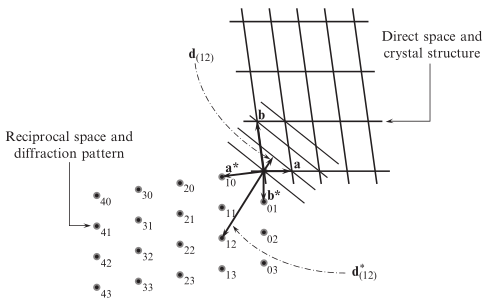
\includegraphics[width=0.6\linewidth]{obr.png}}
%\caption{Пример перехода кристаллографических плоскостей прямой решетки в обратную. Соответствующиие индексы Миллера показаны около точек обратного пространства \cite{spr}}
%\label{obr}
%\end{figure}

Чтобы учесть вклад атомов кристаллической решетки в отражение вводят структурный фактор: \[F(h, k, l) = |F |\cdot e^{i\phi} = \sum_{j=1}^N f_j exp[2\pi i(hx_j + ky_j + lz_j)], \] где $\phi$~---~ фаза отражения, $f_j$~--~ атомный фактор, отражающий вклад атома, $(x_j, y_j, z_j)$~-- координаты атома. Структурный фактор является комплексной величиной. В ходе эксперимента регистрируется интенсивность отражения, отражающая число детектированных рентгеновских лучей, которая равна квадрату модуля структурного фактора $|F|^2$.

Трехмерное распределение атомов в решетке может быть получено только после перехода дифракционной картины из обратного в прямое пространство с помощью Фурье-преобразования: \[\rho(x, y, z) = V^*\sum_{h,k,l} F(h,k,l) exp[(-2\pi i (hx+ky+lz)],\] где $V^*$~-- объем элементарной обратной ячейки \cite{giro}. Как видно из формулы, для расчета электронной плотности требуется структурный фактор, но из эксперимента можно определить только его амплитуду. Данная проблема получила название проблема фаз. Имея достаточный набор отражений, данную проблему можно решить с помощью прямых методов, полагающихся на атомность электронной плотности, или метода Charge flipping.

Получение трехмерной структуры биологических макромолекул является важной задачей для понимания механизма их функций и активности \cite{xrdsap}. Дифракционные картины белков ограничены малыми углами отражения, так как их кристаллы из-за большого количества атомов в ячейке обладают меньшей кристалличностью, чем низкомолекулярные образцы \cite{giro}. Из-за низкого разрешения невозможно определить положения атомов в кристаллической ячейке белка рутинными ab~initio методами, требуется дополнительная информация. Зная аминокислотную последовательность, можно получить структуру белка, если уже известна структура с той же последовательностью, методом молекулярного замещения. Если же такая структура недоступна, то кристаллографическая проблема фаз может быть решена методом изоморфного замещения, в рамках которого проводят дополнительные рентгенодифракционные эксперименты, добавляя тяжелые атомы в структуру \cite{acta}.

Применение машинного обучения в области рентгеновской дифракции лишь недавно зародилось и сейчас бурно развивается. Так, недавняя статья \cite{science} является единственной публикацией по решению проблемы фаз с помощью методов глубокого обучения. В качестве объектов предсказания они выбрали центросимметричные структуры, для которых фазы отражений принимают два возможных значения --- 0 и 1. Авторы презентовали нейронную сеть, представляющую собой бинарный классификатор из блоков трехмерных свёрток и многослойных перцептронов. Обучение проводилось на синтетических кристаллических молекулярных структурах. Также в работе реализована идея phase recycling~--- исходные данные прогоняются несколько раз через модель, что увеличивает точность классификации. Таким образом, впервые был продемонстрирован потенциал машинного обучения для решения проблемы фаз, но только для центросимметричных структур.

Но были найдены решения аналогичной проблемы с помощью методов глубокого обучения в области физики, а именно в рамках метода когерентной безлинзовой микроскопии. В обзорной статье \cite{review_physics} выделены 3 подхода~---~ DL-post-processing, в котором уточняются "плохие фазы", полученные из исходных интенсивностей; DL-in-processing, в рамках которого из интенсивностей с помощью нейронной сети рассчитывают фарзы; и DL-pre-processing, в котором обученная модель повышает разрешение микроскопической картины, и уже из полученного изображения фазы определяются классическими методами.

Таким образом, решение фазовой задачи белковой кристаллографии является актуальной задачей, нерешаемой рутинными методами. Создание инструментов на основе методов глубокого обучения для преодоления данной проблемы является целью работы. 


\subsection*{Данные}

Для генерации данных для обучения использовалось собственное программное обеспечение (\url{github.com/blackwood168/xrd_simulator}), в котором с помощью библиотеки CCTBX (Computational Crystallography Toolbox \cite{cctbx}) создаются кристаллические решетки, в которых случайным образом расставлены атомы, и рассчитываются структурные факторы. Использовались наиболее распространенные для молекулярных кристаллов (набор №1) пространственные группы (P-1, P2$_1$, P$2_1/c$, C2/c, P2$_1$2$_1$2$_1$, Pbca), а также группы моноклинной (P$2_1$, C2) и орторомбической (C222$_1$, P2$_1$2$_1$2, P2$_1$2$_1$2$_1$) сингоний (набор №2, 3), соответствующие наиболее распространенным белковым структурам в базе данных белков (\url{rcsb.org/stats/distribution-space-group}); типы атомов --- C, N, O, Cl; число симметрийно независимых атомов 10--30. Также в работе использовались данные из Кембриджского Банка Структурных Данных \cite{csd}. Высокое разрешение выбрано 0.8 Å, низкое --- 1.5 Å.

В ходе выполнения работы были обучены нейросети, предсказывающие как интенсивность, так и модуль структурного фактора (амплитуду). Типичные распределения этих данных для сгенерированных структур представлено на рис. \ref{F_dist}. Как можно заметить, распределение амплитуд больше похоже на стандартное. Дифракционные данные также были отнормированы в диапазон 0-1.

\begin{figure*}[ht!]
            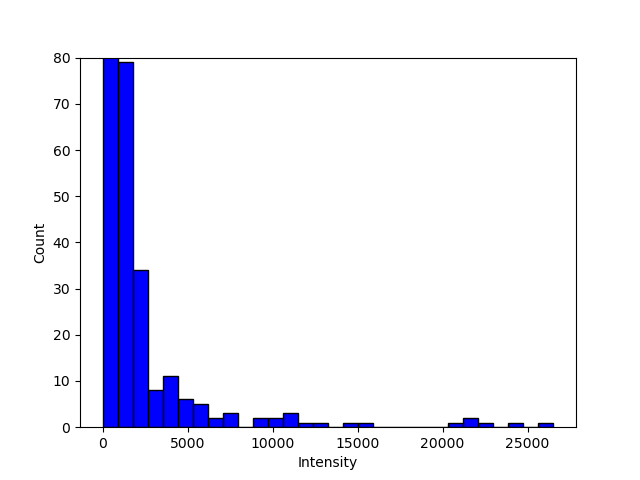
\includegraphics[width=.5\textwidth]{F2_distribution.png}\hfill
            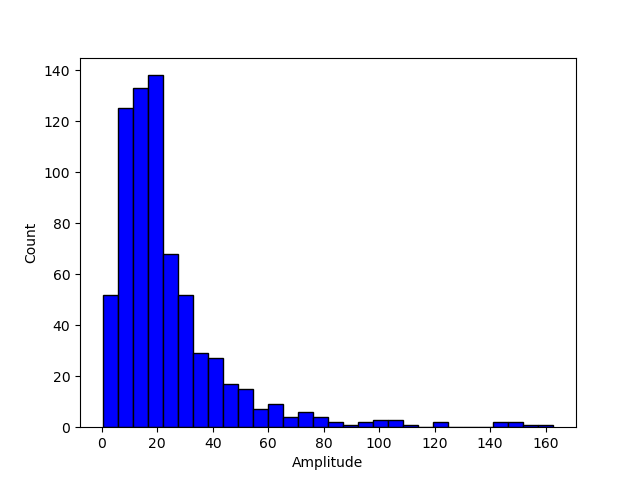
\includegraphics[width=.5\textwidth]{F_distribution.png}
            \caption{Типичные распределения интенсивностей (слева) и амплитуд (справа) дифракционной картины}
            \label{F_dist}
\end{figure*}




\subsection*{Методология}

В работе было предложено предсказывать интенсивности или амплитуды дифракционных отражений белков, которые нельзя получить из эксперимента, по известным из того же эксперимента. После предсказания достаточного количество рефлексов, разрешения должно хватить для определения фаз и расчета электронной плотности одним из рутинных ab initio методов.

Так как отражения являются точками обратного пространства, каждое из них можно однозначно описать индексами Миллера (h,k,l). Тогда дифракционную картину можно описать трехмерным тензором, в котором записаны интенсивности каждого отражения. Таким образом, задача сводится к восстановлению трехмерного тензора. Inference моделей глубокого обучения должен выглядеть следующим образом: на вход подается тензор с рентгенодифракционными экспериментальными данными, на выходе должен быть тензор с дополнительными интенсивностями. В ходе обучения планируется научить модель восстанавливать тензор отражений по данным малых органических молекул. Для этого будут обнулены интенсивности дальних отражений так, чтобы длина разрешения полученной дифракционной картины соответствовала типичному разрешению белковых соединений (1.5 Å).

В качестве моделей были предложены и проверены вариационный автоэнкодер и сверточная сеть UNet, адаптированные под трехмерные матрицы. Рассматривается также использование архитектур типа трансформеры, механизм внимания которых может быть полезен для данной задачи.

Эффективность предсказания обученных моделей глубокого обучения предлагается проверять на тестовой части синтетического датасета, а также собранных наборах экспериментальных данных.

В ходе выполнения работы также предложен постпроцессинг, включающий в себя учёт систематических погасаний --- "зануления" некоторых значений интенсивностей, что определяется симметрией структуры; а также явного восстановления части тензора, которую не нужно предсказывать.


\subsection*{Результаты}

В рамках данной работы был разработан пайплайн, позволяющий проводить воспроизводимые эксперименты (\url{github.com/blackwood168/xrd_phase_ml}). В нем реализовано обучение и тестирование моделей, а также inference на реальных массивах данных и структурах кристаллических соединений.


\subsubsection*{Наивный подход}

По набору №1 структур, пространственные группы которых соответствуют наиболее распространенным для молекулярных кристаллов, были обучены UNet и вариационный автоэнкодер (рис. \ref{UVAE_ALL}). Модели были обучены на датасете из 40 тысяч структур. На вход подавалась матрица интенсивностей дифракционных картин, архитектуры моделей были адаптированы под трехмерный случай. Значение среднеквадратичной ошибки на синтетической отложенной тестовой выборке составляет 16.1$\cdot$10$^{-5}$ и 1.05$\cdot$10$^{-5}$ для VAE и UNet, соответственно. Можно сделать вывод, что адаптированная архитектура UNet лучше справляется с восстановлением дифракционной картины.

\begin{figure*}[ht!]
            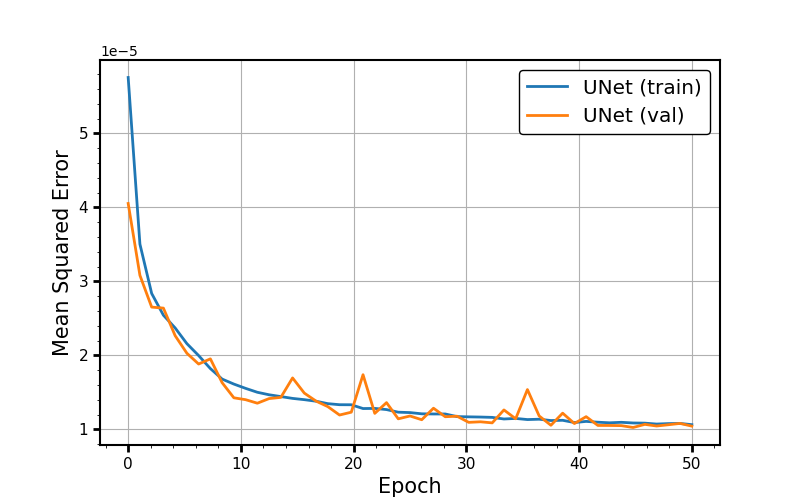
\includegraphics[width=.5\textwidth]{UNet_all.png}\hfill
            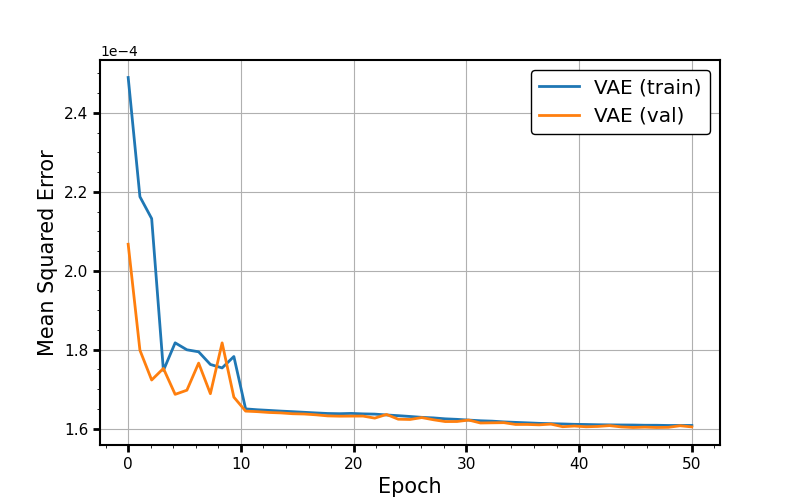
\includegraphics[width=.5\textwidth]{VAE_all.png}
            \caption{Кривые обучения для UNet (слева) и VAE (справа)}
            \label{UVAE_ALL}
\end{figure*}

В ходе анализа данного подхода выяснилось, что он имеет ряд недостатков. Так, модели не выучивают паттерны систематических погасаний, от чего тензор интенсивностей не имеет нулевых значений. Также модели не сохраняют интенсивности ближних отражений, то есть центра тензора, по которому происходит восстановление в ходе inference. 

Самым же важным недостатком является то, что для описания дифракционных картин требуются матрицы размером 33x36x29, но для большинства структур они будут сильно разрежены. Связано это с тем, что в дифракционные данные попадают только симметрично независимые отражения. У более симметричных структур будет меньше независимых отражений, и наоборот. Это приводит к тому, что для структур с высокой симметрией большая часть  данных заполнена нулями. Поэтому имеет смысл обучать разные модели для каждой рассматриваемой кристаллической сингонии, чтобы избежать разреженных матриц.

\subsubsection*{Моноклинная сингония}

По набору №2 структур моноклинной сингонии были обучены разные модели UNet (рис. \ref{UCLIN}). Размер матриц для данной сингонии 26x18x23. Обучение происходило на датасете из 60 тысяч образцов и большом датасете на 200 тысяч. Также варьировался размер модели, в большой модели на 1 вертикальный блок больше.

\begin{figure*}[]
            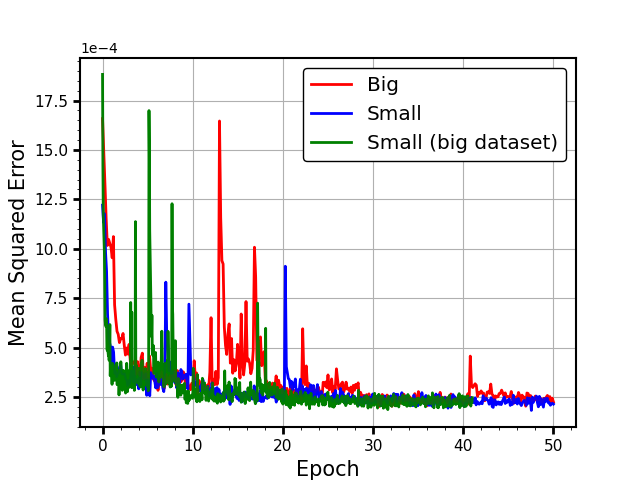
\includegraphics[width=.5\textwidth]{Train_clin.png}\hfill
            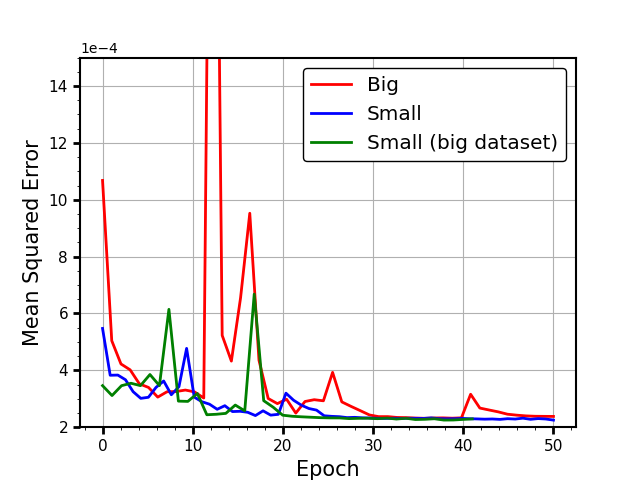
\includegraphics[width=.5\textwidth]{Val_clin.png}
            \caption{Тренировочная (слева) и валидационная (справа) кривые обучения}
            \label{UCLIN}
\end{figure*}

Значение MSE на отложенной тестовой выборке представлены в таблице \ref{tabl1}, MSE-Postprocessing --- значение среднеквадратичной ошибки, после применения постпроцессинга к восстановленным матрицам. Можно сделать вывод, что восстанавливающая способность моделей отличается незначительно. Наилучший же результат показывает маленькая модель, обученная на большом датасете (200 тысяч структур).

\begin{table}
\centering
\captionof{table}{Значения среднеквадратичной ошибки на отложенной тестовой выборке} 
\begin{tabular}{|c|c|c|}
\hline
\label{tabl1}
\textbf{Модель}                                                       & \textbf{MSE$\cdot$10$^{-5}$} & \textbf{MSE-Postprocessing$\cdot$10$^{-5}$} \\ \hline
Маленькая                                                             & 22.75                  & 22.64                                   \\ \hline
Большая                                                               & 23.35                  & 23.14                                   \\ \hline
\begin{tabular}[c]{@{}c@{}}Маленькая, \\ большой датасет\end{tabular} & 22.46                  & 22.33                                   \\ \hline
\end{tabular}
\end{table}



\subsubsection*{Орторомбическая сингония}

По набору №3 структур орторомбической сингонии была обучена модель с архитектурой UNet (рис. \ref{ROMB}). Обучение происходило на датасете из 60 тысяч структур, размер матриц составил 17x22x29. На отложенной тестовой выборке значения ошибки составили 20.37$\cdot$10$^{-5}$ и 20.26$\cdot$10$^{-5}$ до и после постпроцессинга, соответственно.

\begin{figure}[H]
	\center{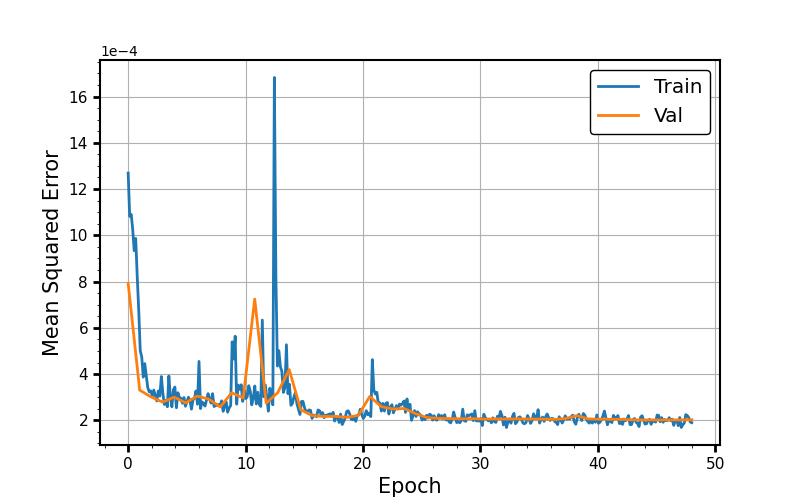
\includegraphics[width=0.7\linewidth]{2layers_romb.png}}
	\caption{Кривые обучения}
	\label{ROMB}
\end{figure}

\subsubsection*{Проверка на реальных данных}

Было проведено тестирование на реальных молекулярных моноклинных структурах из Кембриджского Банка Структурных данных \cite{csd}. Среднее значение MeanAbsoluteError по результатам тестирования на 60 структурах составило 0.0013. Далее восстановленная нейронной сетью матрица подавалась на вход в кристаллографические программы для решения структур ShelXT и ShelXL. Однако ни одну структуру по восстановленным данным не получилось решить. 


\subsection*{Выводы}

\begin{itemize}
\item Разработано программное обеспечение по генерации синтетических рентгенодифракционных данных (\url{github.com/blackwood168/xrd_simulator})

\item Разработан единый пайплайн (\url{github.com/blackwood168/xrd_phase_ml}), позволяющий проводить воспроизводимые эксперименты

\item Обучены вариационный автоэнкодер и UNet на кристаллических структурах различной сингонии, лучшую эффективность продемонстрировала UNet

\item Обучены сверточные нейронные сети с архитектурой UNet для структур орторомбической и моноклинной сингоний

\item Проведено тестирование на реальных рентгенодифракционных данных на предмет возможности решения структуры по восстановленным данным

\end{itemize}
}
\sloppy{
\addcontentsline{toc}{subsection}{Список литературы}
%\bibliographystyle{gost71s}
%\bibliographystyle{utf8gost705u}
%\bibliographystyle{utf8gost71s}
%\bibliographystyle{gost2008}
\bibliographystyle{gost2008l}
\bibliography{lit}

}
\end{document}
